\documentclass[oneside,a4paper]{article}
\usepackage{subfig}
\usepackage{graphicx}
\usepackage{hyperref}
\usepackage{tabularx}
\usepackage{tabulary}
\usepackage[dvipsnames]{xcolor}
\usepackage{colortbl}
\usepackage[official]{eurosym}
\usepackage[margin=1.5in]{geometry}    % For margin alignment
\usepackage[english]{babel}
\usepackage[utf8]{inputenc}
\usepackage{algorithm}
\usepackage{amssymb}
\usepackage{arevmath}     % For math symbols
\usepackage[noend]{algpseudocode}
\algdef{SE}[VARIABLES]{Variables}{EndVariables}
   {\algorithmicvariables}
   {\algorithmicend\ \algorithmicvariables}
\algnewcommand{\algorithmicvariables}{\textbf{global variables}}
\algnewcommand\algorithmicforeach{\textbf{for each}}
\algdef{S}[FOR]{ForEach}[1]{\algorithmicforeach\ #1\ \algorithmicdo}
\algdef{SE}[SUBALG]{Indent}{EndIndent}{}{\algorithmicend\ }%
\algtext*{Indent}
\algtext*{EndIndent}
%margins
\setlength\textwidth{16.5cm}      %
\setlength\textheight{22.7cm}     % [a4: 21cm x 29.7cm]
\setlength\oddsidemargin{-0.4cm}  %
\setlength\topmargin{-2.5cm}        %
\setlength\footskip{1.5cm}          %
%
\usepackage{bera}% optional: just to have a nice mono-spaced font
\usepackage{listings}
\usepackage{xcolor}

\colorlet{punct}{red!60!black}
\definecolor{background}{HTML}{EEEEEE}
\definecolor{delim}{RGB}{20,105,176}
\colorlet{numb}{magenta!60!black}

\lstdefinelanguage{json}{
    basicstyle=\normalfont\ttfamily,
    numbers=left,
    numberstyle=\scriptsize,
    stepnumber=1,
    numbersep=8pt,
    showstringspaces=false,
    breaklines=true,
    frame=lines,
    backgroundcolor=\color{background},
    literate=
     *{0}{{{\color{numb}0}}}{1}
      {1}{{{\color{numb}1}}}{1}
      {2}{{{\color{numb}2}}}{1}
      {3}{{{\color{numb}3}}}{1}
      {4}{{{\color{numb}4}}}{1}
      {5}{{{\color{numb}5}}}{1}
      {6}{{{\color{numb}6}}}{1}
      {7}{{{\color{numb}7}}}{1}
      {8}{{{\color{numb}8}}}{1}
      {9}{{{\color{numb}9}}}{1}
      {:}{{{\color{punct}{:}}}}{1}
      {,}{{{\color{punct}{,}}}}{1}
      {\{}{{{\color{delim}{\{}}}}{1}
      {\}}{{{\color{delim}{\}}}}}{1}
      {[}{{{\color{delim}{[}}}}{1}
      {]}{{{\color{delim}{]}}}}{1},
}
\usepackage{authblk}
\usepackage{tabu}
\usepackage{tabularx}
\usepackage{ltablex}
\usepackage{longtable}
\usepackage{float} % To allow the use of H modifier in long tables
%landscape mode
\usepackage{pdflscape}
\usepackage{rotating}
\usepackage{caption}
\providecommand{\keywords}[1]{\textbf{\textit{Keywords:}} #1}
\title{Title of the article}
\author{Giuseppe Sorrentino, Marco Tonnarelli, Marco Venere}
\affil{Politecnico di Milano\\
Milan, Italy\\
\href{mailto:first.last@polimi.it}{{ giuseppe.sorrentino@mail.polimi.it\\}{marco.tonnarelli@mail.polimi.it\\} {marco.venere@mail.polimi.it} }}
\date{}

\begin{document}
\maketitle
\begin{abstract}
Abstract of the paper. Abstract of the paper. Abstract of the paper. Abstract of the paper. Abstract of the paper. Abstract of the paper. Abstract of the paper. Abstract of the paper. Abstract of the paper. Abstract of the paper. Abstract of the paper. Abstract of the paper. Abstract of the paper. Abstract of the paper. Abstract of the paper. Abstract of the paper. Abstract of the paper. Abstract of the paper. Abstract of the paper. Abstract of the paper. Abstract of the paper. Abstract of the paper. Abstract of the paper. Abstract of the paper. Abstract of the paper. Abstract of the paper. Abstract of the paper. Abstract of the paper. Abstract of the paper. Abstract of the paper. Abstract of the paper. Abstract of the paper. Abstract of the paper. Abstract of the paper. Abstract of the paper.
\end{abstract}

\keywords{one, two, three, four}

\section{Introduction}
Over the past forty years, the frontiers of computer science are focused on developing more and more effective machines with an extremely high computational power: quantum computers. From the very beginning of the ‘80s, when Paul Benioff proposed the first model of the quantic touring machine, several improvements have been reached. Nowadays, one of the most promising machines is the quantum annealer, which aims to heuristically solve difficult combinatorial optimization problems\cite{WebSite3}. To show the possibilities of this technology, in the present article a possible solution for the Set Packing Problem is shown. Even if it is extremely famous in literature and several solutions have been proposed using classical computers, in the algorithm presented later two different kinds of quantum annealers have been used and their results have been compared.
To execute the algorithm, the quantum annealers of D-Wave have been used \cite{article1}.In particular, we used Leap,a real-time Quantum Application Environment. It is a cloud-based platform giving application developers real-time access to a quantum computer. Here, two powerful quantum annealers are available: the 2000Q and the Advantage. They are controllable supercomputer that works at extremely low temperature. In particular: 
\begin{itemize}
    \item \textbf{The dwave-hybrid} framework.
    \item \textbf{the 2000Q} has a footprint of approximately 10' x 7' x 10' (L x W x H). Its physical enclosure houses sophisticated cryogenic refrigeration, shielding, and I/O systems to support a single thumbnail-sized QPU.  Most of the physical volume of the system is required to accommodate the refrigeration system 
and to provide easy service access.  For quantum effects to play a role in computation, the QPU requires an extreme, isolated environment. It works at a temperature of 15 mK and it has up to 2048 qubits and 6016 couplers.
    \item \textbf{the Advantage} system is the first and only quantum computer designed for business. 
    It is the 5th generation Advantage quantum computer that was built from the ground up with 
    a new processor architecture with over 5,000 qubits and 15-way qubit connectivity, empowering enterprises to solve their largest and most complex business problems. The main strength of the advantage Is the higher number of qubits, which makes it computationally more powerful than the 2000Q while the main drawback is the high noise which affects its data.
\end{itemize}
In addition to supercomputers, in the first phase of the project, we used also the Dwave-hybrid sampler \cite{WebSite6} in order to test the algorithm. Essentially, it is a framework which allows solving an optimization problem by decomposing it into two or more solutions which run in parallel. These solutions, using the D-Wave hybrid sampler, may or may not involve the supercomputers previously mentioned. The use of this framework allowed us to be sure about the feasibility of the algorithm. Then, we left the hybrid framework to focus on 2000Q and Advantages exclusively.
In the first section of this paper, the Set Packing Problem the specific formalization provided by Glover for quantum computing\cite{Website1} is better described. Then, there is a description of the algorithm and of the formal descriptive paradigm used. The format described was essential to implement a problem generator for testing. After this, in the third part of the paper, the results of our experiment have been shown to highlight the effectiveness of both machines while in the last part there is a comparison between them to put a spotlight on the strengths and drawbacks.

\section{The Set Packing Problem}


The focus of our research is the set packing problem. It is a combinatorial optimization problem which has been extensively studied in the past recent years[]. The formulation of the problem is the following: given a set of n finite sets, a packing is a collection of all the sets among the n ones which are mutually disjoint. The main objective of the problem is to find the packing of the maximum size[]. Set packing is an NP-hard maximization problem. Here follows the problem formalization given by Glover []:


\centerline{${ max {\sum_{j=1}^{n}w_jx_j}}$}
\centerline{
st
}

\centerline{${\sum_{j=1}^{n}a_ijxj \leq 1 \forall j \in 1..m}$}

\setlength\parindent{0pt}where ${a_ij}$ are 0/1 coefficients, ${w_j}$ are weights and ${x_j}$ variable are binary.



\setlength\parindent{10pt}In order to make the algorithm work on the quantum annealer, it is necessary to reformulate the problem as a QUBO model, which is the acronym of Quadratic Unconstrained Binary Optimization problem. The QUBO model is a special framework specifically designed for Combinatorial Optimization problems. In these kind of problems, a large number of decision must be made and these decisions yield to a corresponding objective function value. QUBO models belong to the class of NP-hard problems. For this reason, finding the optimal solution of such a problem might be unfeasible as the size of the instance increases. However, it is possible to find very good but not necessarily optimal solution in a reasonable amount of computational time.
The idea behind the QUBO formulation is use the following objective function:\\
\centerline{${minimize/maximize\; y = x^tQx}$}\\
where x a vector of binary decision variables and Q is a square matrix (symmetric or upper triangular) of constraints. The constraints of a traditional optimization problem become, in the QUBO model, a set of quadratic penalties introduced in the previously mentioned objective function. The penalties are structured in a way that they are equal to zero for feasible solutions or equal to some positive amount for unfeasible solutions. For the Set Packing problem, we obtained the following QUBO representation: \centerline{${max\; x^tQx}$}.

In order to achieve our objectives, we implemented the set packing problem using the Leap platform provided by D-wave systems, where we used a built in function which is able to map a traditional optimization problem into a QUBO model in such a way that it can be run on the quantum annealer.

\section{The Algorithm}
The definition of the algorithm for the solution of a generic Set Packing problem has been based on the platform and libraries developed by D-Wave (i.e., Leap IDE [] and D-Wave System respectively). The testing has been focused on two different quantum annealers: 2000Q and Advantage.

Firstly, it was necessary to define a formal descriptive paradigm of a Set packing problem, able to rigorously express all the subsets belonging to the set and the related constraints, according to the Grover formalization. 

Secondly, the first phase of the development of the algorithm has started, in which the code has been tested on a single instance of the problem, for both architectures, and the spatial and time complexities have been analysed.

Subsequently, the second phase has taken place, in which the parameters of the algorithm have been tuned by executing several experiments, for both architectures. Spatial and time complexities have been studied, and compared to the previous ones. 
\subsection{The problem format and generator}
In order to elaborate an effective algorithm for the solution of a generic Set Packing problem, a formal paradigm has been defined, aiming at describing the instance of the problem, with the subsets and their weights, as well as all the constraints that exist among them.

During the definition of such a format, priority has been given to two important language characteristics:
\begin{enumerate}
    \item \textbf{expressiveness}: the chosen language should be able to express, in a clear and concise way, all the features of the problem, so as to be, at the same time, human-readable and unambiguous;
    \item \textbf{scripting-compliance}: the chosen language should be thoroughly supported by the standard libraries of the majority of the scripting languages, in order to ease its use and spreading. In addition, being scripting-compliant also reduces the probability of the presence of vulnerabilities and errors in the code related to translation, for standard libraries are widely tested against such risks;
    \item \textbf{parsing speed}: the chosen language should be parsable very fast, as it will be used very extensively.
\end{enumerate}
After an extensive analysis, it has been decided that the most convenient format to adopt is JSON (JavaScript Object Notation, []), as it is strongly expressive, widely supported by the majority of scripting languages, and parsable at high velocity [\url{https://lemire.me/blog/2018/05/03/how-fast-can-you-parse-json/}].

In particular, the generic format is defined as an array of objects, each of which describes an instance of a problem. The usage of arrays allows for multiple instances to be considered at the same time. Each of these objects contains two fields: \textit{subsets}, which is an array of the subsets belonging to the set, and \textit{constraints}, which is an aray of the constraints among the subsets. 

The subsets are defined as object, containing a \textit{name}, which is a string, and a \textit{weight}, which is a number, and is optional (its default value is 1). The constraints are objects as well, containing an attribute \textit{sets}, that is an array of string, each referring to a previously defined set.

An example of an instance of the problem is the following: 

\begin{lstlisting}[language=json,firstnumber=1]
[{
    "subsets": 
        [
            {"name": "1E8", "weight": 8},
            {"name": "Z7MF"},
            {"name": "F", "weight": 6},
            {"name": "B", "weight": 6},
            {"name": "1MS8", "weight": 5},
            {"name": "ZI"}
        ],
    "constraints":
        [
            {"sets": ["B", "ZI"]},
            {"sets": ["1MS8", "ZI", "F"]},
            {"sets": ["1E8", "B", "Z7MF", "F", "1MS8", "ZI"]}
        ]
}]
\end{lstlisting}

Once the format has been defined, a script has been written in order to generate random instances of a set packing problem. Since, for complexity analysis, it is necessary to control the size of the instance (i.e., the number of subsets considered in the problem), such a parameter is the input of the script. The procedure returns a file containing the instance of the problem, written as the format described above prescribes.

\begin{algorithm}
\caption{Set Packing Problem generator}
\begin{algorithmic}[1]

\Procedure{GenerateSetPackingProblem}{$filename$, $N$}      

    \State set S := $\varnothing$  \Comment{Set of subsets names}
    \State set W := $\varnothing$  \Comment{Set of subsets weights}
    \State set C := $\varnothing$  \Comment{Set of constraints}
    \While{size(S) $\not=$ $N$ } 
        \State S $\leftarrow$ random$\_$string()   \Comment{Create random subset name}
        \State W $\leftarrow$ random$\_$number$\_$or$\_$null()  \Comment{Create random optional subset weight}
    \EndWhile  \label{loop}
    \State int size$\_$of$\_$C $\leftarrow$ random$\_$positive$\_$up$\_$to$\_$($N$)  \Comment{generate random size of C}
    \While{size(C) $\not=$ size$\_$of$\_$C}  
        \State C $\leftarrow$ random$\_$constraint$\_$from$\_$subsets(S) \Comment{Create random constraint from defined subsets}
    \EndWhile  \label{loop1}
    \State json J $\leftarrow$ create$\_$JSON(S, W, C)  \Comment{Create JSON object from given sets, by using defined format} 
    \State file F $\leftarrow$ create$\_$file($filename$, J);  \Comment{Create file with content J}
    \State \Return F  \Comment{return file}
\EndProcedure

\end{algorithmic}
\end{algorithm}
Thanks to this generator, it has been possible to automatically generate several instances of the problem, of different sizes, in order to evaluate the space and time complexity of the algorithm for the resolution of the problem. 
\subsection{The first phase}
In the first phase of the development of the algorithm, a study of the D-Wave Leap IDE platform has been performed, and the Python programming language has been used, since it is the language chosen by the D-Wave environment. 

The Set Packing problem has been modeled as an object of the Set Packing class, which embodies all the data related to subsets and constraints, and paves the way for the usage of the \textit{BinaryQuadraticModel}, that is the main representation of a Binary Quadratic Model in the D-Wave System library. In particular, all the subsets are represented as \textit{variables} of the problem, and the constraints as \textit{interactions} among variables.

After the program is correctly represented in memory, the sampling stage begins, by choosing one of the three topologies on which this study is based:
\begin{enumerate}
    \item \textit{2000Q}: It is invoked by the \textit{EmbeddingComposite} object, by specifying \textit{chimera} as topology type.
    \item \textit{Advantage}: it is invoked by the \textit{EmbeddingComposite} object, as a default choice, thus no topology type needs to be specified.
    \item \textit{Hybrid}: it is invoked by the \textit{LeapHybridSampler} object. It is an hybrid architecture.
\end{enumerate}

Once the sampler has been chosen, the sampling stage can take place, and its results, received as a sampleset, can ben analyzed. The platform allows the use of a specific tools, called \textit{Inspector}, made available for the 2000Q and Advantage architectures, that let developers visualize the problems received from the machine and control several parameters, in addition to the quantum bits involved in the computation. Such parameters have been considered for the evaluation of the space and time complexity of the algorithm, and because of the absence of an inspector screen for the \textit{LeapHybridSampler}, for such a topology it is not possible to show any computational trend.

As a matter of completeness, the pseudocode of the resolution of a set packing problem is here reported. The input of the \textit{SolveSetPackingProblem} is a file name, corresponding to a file that has been previously written in accordance to the aforementioned format.

\begin{algorithm}
\caption{Set Packing Problem solver}
\begin{algorithmic}[1]
\Require a file with name $filename$, consistent with the defined format
\Procedure{SolveSetPackingProblem}{$filename$, $N$} 
\State \textbf{parameters}
\Indent
    \State $penalty$: the penalty associated to the violation of a constraint
    \State $sampler$: the sampler, and related solver, associated to the desired architecture.
\EndIndent
\State \textbf{end parameters}
\Variables
 \State $P$, SetPackingProblem
 \State $bqm$, BinaryQuadraticModel
\EndVariables
%read file
\State $P$ := read$\_$sanitized$\_$file($filename$)  \Comment{Read a file, and verify if the format is consistent and instantiate the corresponding SetPackingProblem}
\ForEach {subset $\in$ $P$.subsets} 
        \State $bqm$.add$\_$variable(subset.name, subset.weight)   \Comment{Add subset and its weight as a variable into the binary quadratic model}
\EndFor  \label{loop2}
\ForEach {constraint $\in$ $P$.constraints} 
    \ForEach {i $\in$ constraint}
        \ForEach {j $\in$ constraint, j $<$ i}
            \State $bqm$.add$\_$interaction(i, j, $penalty$)   \Comment{Add an interaction for each pair of sets in a constraint}
        \EndFor
    \EndFor
\EndFor  \label{loop3}
\State sampleset := $sampler$.sample($bqm$) \Comment {Sample the binary quadratic model with $sampler$}
\State show$\_$inspector(sampleset) \Comment {Show the inspector for the sampleset, if available}
\State \Return sampleset \Comment{Return the sampleset}
\EndProcedure
\end{algorithmic}
\end{algorithm}

\textbf{2000Q: space and time complexity} \\

For what concerns the 2000Q architecture, the maximum size of a set packing problem that has been successfully computed is circa 60. In order to consider the space complexity, the inspector has been checked for increasing sizes of the problem ($N$ = 10, 20, 30, 40, 50, 60). For these values, the maximum chain length has been reported.



\begin{figure}[htp]
\begin{minipage}[b]{4.5cm}

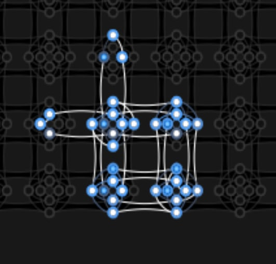
\includegraphics[width=5cm]{LaTeXTemplate/Images/2000Qfirst10.png}
\caption{N=10\\max chain length = 4}
\end{minipage}
\ \hspace{2mm} \hspace{2mm} \
\begin{minipage}[b]{4.5cm}

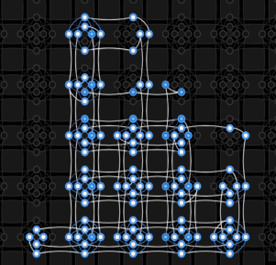
\includegraphics[width=5cm]{LaTeXTemplate/Images/2000Qfirst20.png}
\caption{N=20\\max chain length = 7}
\end{minipage}
\ \hspace{2mm} \hspace{2mm} \
\begin{minipage}[b]{4.5cm}
\centering
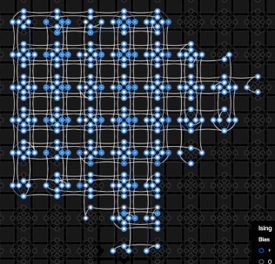
\includegraphics[width=5cm]{LaTeXTemplate/Images/2000Qfirst30.png}
\caption{N=30\\max chain length = 12}
\end{minipage}
\end{figure}

\begin{figure}[htp]
\begin{minipage}[b]{4.5cm}
\centering
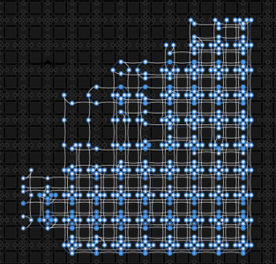
\includegraphics[width=5cm]{LaTeXTemplate/Images/2000Qfirst40.png}
\caption{N=40\\max chain length = 15}
\end{minipage}
\ \hspace{2mm} \hspace{2mm} \
\begin{minipage}[b]{4.5cm}
\centering
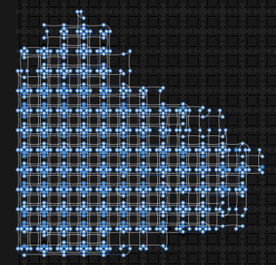
\includegraphics[width=5cm]{LaTeXTemplate/Images/2000Qfirst50.png}
\caption{N=50\\max chain length = 21}
\end{minipage}
\ \hspace{2mm} \hspace{2mm} \
\begin{minipage}[b]{4.5cm}
\centering
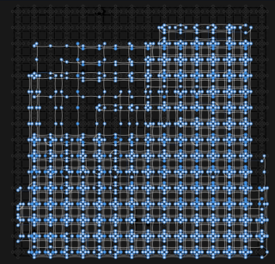
\includegraphics[width=5cm]{LaTeXTemplate/Images/2000Qfirst60.png}
\caption{N=60\\max chain length=31}
\end{minipage}
\end{figure}

In order to evaluate the time complexity of the algorithm, it has been tested on increasing sizes of the problem, and the QPU time spent by the machine (i.e., the time spent by the QPU to solve the problem, [\url{https://docs.dwavesys.com/docs/latest/c_qpu_timing.html]}) has been analyzed. The following plots show the trends of the time complexity:
\begin{figure}[htp]
\centering
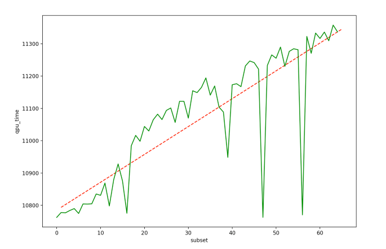
\includegraphics[width=15cm]{LaTeXTemplate/Images/2000QfirstT1.png}
\caption{Time complexity, with outliers (real values in green, general trend in red)}
\end{figure}
\begin{figure}[htp]
\centering
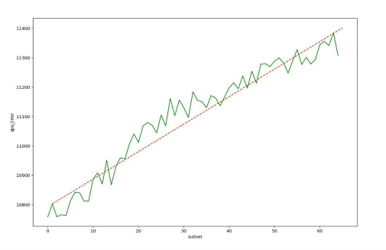
\includegraphics[width=15cm]{LaTeXTemplate/Images/2000QfirstT2.png}
\caption{Time complexity, without outliers (real values in green, general trend in red)}
\end{figure}

In figure 7, it can be notice that the overall trend is a linear increase, even though some spikes are present, due to the intrinsic noise belonging to the machines. By removing such outliers, the linearity is even more noticeable, as figure 8 shows.
\\
\\
\textbf{Advantage: space and time complexity} \\

Analogous considerations have been made for the Advantage architecture. In this case, the maximum size for an instance to be successfully computed is about 150. The space complexity has been observed for $N$ = 10, 40, 70, 100, 130, 150.

\begin{figure}[htp]
\begin{minipage}[b]{4.5cm}

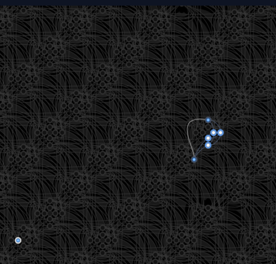
\includegraphics[width=5cm]{LaTeXTemplate/Images/Advantagefirst10.png}
\caption{N=10\\max chain length = 2}
\end{minipage}
\ \hspace{2mm} \hspace{2mm} \
\begin{minipage}[b]{4.5cm}

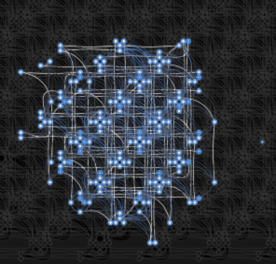
\includegraphics[width=5cm]{LaTeXTemplate/Images/Advantagefirst40.png}
\caption{N=40\\max chain length = 7}
\end{minipage}
\ \hspace{2mm} \hspace{2mm} \
\begin{minipage}[b]{4.5cm}
\centering
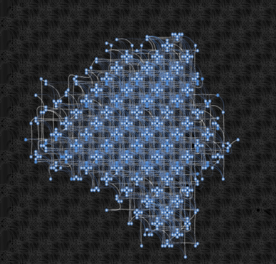
\includegraphics[width=5cm]{LaTeXTemplate/Images/Advantagefirst70.png}
\caption{N=70\\max chain length = 13}
\end{minipage}
\end{figure}

\begin{figure}[htp]
\begin{minipage}[b]{4.5cm}
\centering
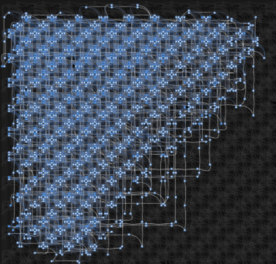
\includegraphics[width=5cm]{LaTeXTemplate/Images/Advantagefirst100.png}
\caption{N=100\\max chain length = 29}
\end{minipage}
\ \hspace{2mm} \hspace{2mm} \
\begin{minipage}[b]{4.5cm}
\centering
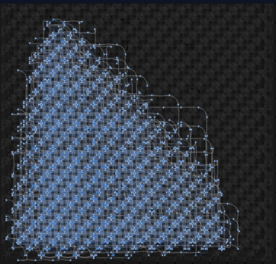
\includegraphics[width=5cm]{LaTeXTemplate/Images/Advantagefirst130.png}
\caption{N=130\\max chain length = 29}
\end{minipage}
\ \hspace{2mm} \hspace{2mm} \
\begin{minipage}[b]{4.5cm}
\centering
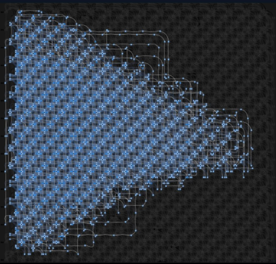
\includegraphics[width=5cm]{LaTeXTemplate/Images/Advantagefirst150.png}
\caption{N=150\\max chain length=32}
\end{minipage}
\end{figure}


In order to evaluate time complexity, the same plots as for the 2000Q architecture have been taken.

\begin{figure}[htp]
\centering
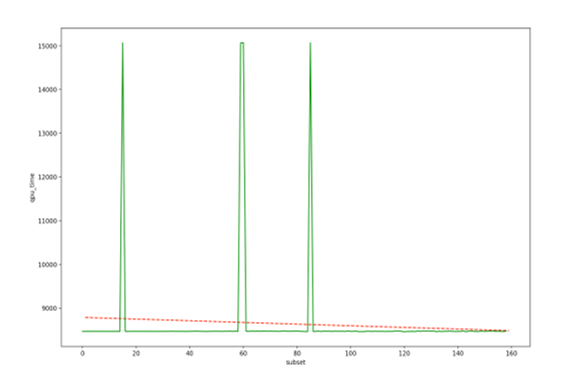
\includegraphics[width=15cm]{LaTeXTemplate/Images/AdvantagefirstT2.png}
\caption{Time complexity, with outliers (real values in green, general trend in red)}
\end{figure}
\begin{figure}[htp]
\centering
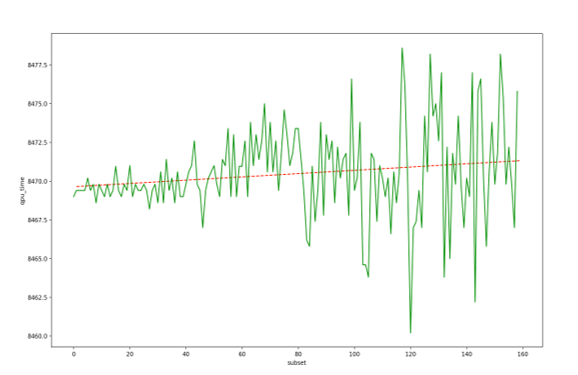
\includegraphics[width=15cm]{LaTeXTemplate/Images/AdvantagefirstT1.png}
\caption{Time complexity, without outliers (real values in green, general trend in red)}
\end{figure}

As figure 15 shows, the presence of some particular spikes prevents a correct analysis of the general trend, due to the noise of the Advantage. By removing such outliers, as in figure 16, 
there can be observed a general linear increase, even though, once again, the great amount of noise of the architecture produces a more irregular pattern.
\newpage

\subsection{The second phase}
After the first phase, in which the algorithm and the problem generator have been tested, we focused on improving the simulations and the experiments modelling some useful parameters. In particular, we modelled the following parameters:\\
\begin{itemize}
    \item \textbf{the num$\_$reads} parameter. It represents the number of samples asked to the solver. By default, it is set to 1 so the solver tries to find just one sample. To get a more reliable result, we set this param to 100.
    \item \textbf{the chain$\_$strength} parameter. It represents the strength of the chain. For the sake of clarity, let us specify that a solution is said to be correct and trustable if it has the least chain breaks possible. Considering this, the chain$\_$strength parameter “forces” the solver to find a solution which is at least as strong as specified. It must be specified that choosing a too low or too high value of chain strength has negative effects. In particular, a too low value leads to a too high number of chain breaks while a too high value leads to a change the nature of the problem\cite{WebSite4}. So, to choose a proper way the value, we used the method uniform$\_$torque$\_$compensation \cite{WebSite5}, which computes the chain strength that attempts to compensate for the torque that would cause the chain breaks.
    \item \textbf{pre$\_$factor} parameter. It is a parameter of uniform$\_$torque$\_$compensation and it allows the method to find the best value of chain$\_$strength. By default, its value is set to 1.414 but, normally, it belongs to a range [0.5,2.0]. By doing several experiments, the optimal value for which the minimum number of chain breaks resulted is 2.0.\\
\end{itemize}
Following, the result of the experiment performed are presented in order analyze the spacial complexity of each instances. 
The problem with a number of subsets belonging to [1,60] have been solved with 2000Q and Advantage while the problem with a number of subsets belonging to [61,150] have been solved with Advantage only since the problems were computationally too hard.\\
\\
\textbf{2000Q : number of chain breaks = 0}
\begin{figure}[htp]
\begin{minipage}[b]{4.5cm}
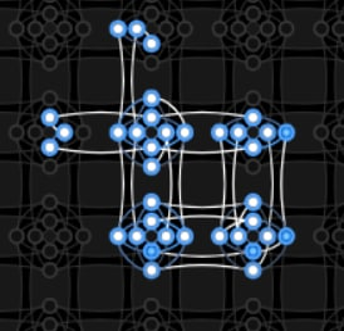
\includegraphics[width=5cm]{LaTeXTemplate/Images/2000QN10.png}
\caption{N=10\\max chain length = 4\\max chain strength=120.72\\physical qubits = 33}
\end{minipage}
\ \hspace{2mm} \hspace{2mm} \
\begin{minipage}[b]{4.5cm}
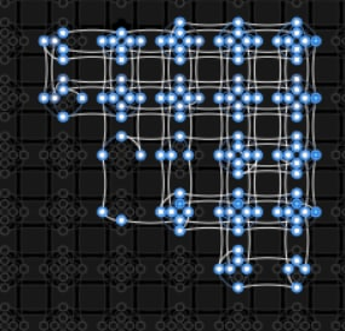
\includegraphics[width=5cm]{LaTeXTemplate/Images/2000QN20.png}
\caption{N=20\\max chain length = 8\\max chain strength=95.47\\physical qubits = 132}
\end{minipage}
\ \hspace{2mm} \hspace{2mm} \
\begin{minipage}[b]{4.5cm}
\centering
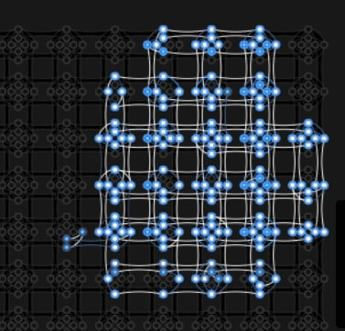
\includegraphics[width=5cm]{LaTeXTemplate/Images/2000QN30.png}
\caption{N=30\\max chain length = 9\\max chain strength=52.21\\physical qubits = 178}
\end{minipage}
\end{figure}
\begin{figure}[htp]
\begin{minipage}[b]{4.5cm}
\centering
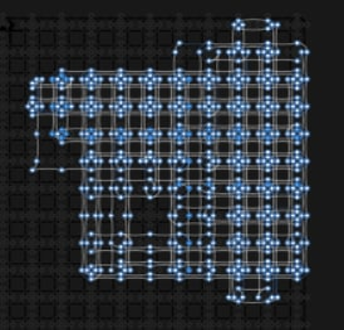
\includegraphics[width=5cm]{LaTeXTemplate/Images/2000QN40.png}
\caption{N=40\\max chain length = 17\\max chain strength=273.18\\physical qubits = 528}
\end{minipage}
\ \hspace{2mm} \hspace{2mm} \
\begin{minipage}[b]{4.5cm}
\centering
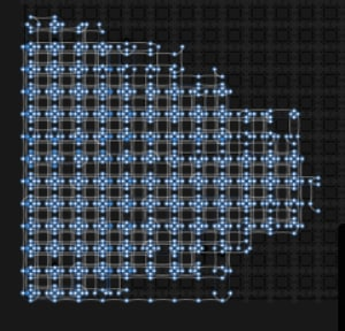
\includegraphics[width=5cm]{LaTeXTemplate/Images/2000QN50.png}
\caption{N=50\\max chain length = 25\\max chain strength=701.68\\physical qubits = 888}
\end{minipage}
\ \hspace{2mm} \hspace{2mm} \
\begin{minipage}[b]{4.5cm}
\centering
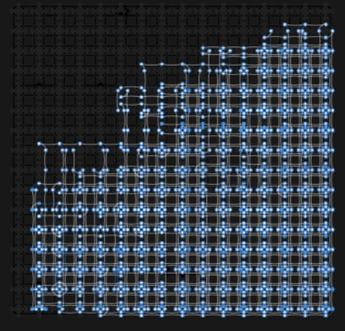
\includegraphics[width=5cm]{LaTeXTemplate/Images/2000QN60.png}
\caption{N=60\\max chain length=33\\max chain strength=1285.3\\physical qubits=1295}
\end{minipage}
\end{figure}
\newpage
\textbf{The Advantage: number of chain breaks = 0}
\begin{figure}[htp]
\begin{minipage}[b]{4.5cm}
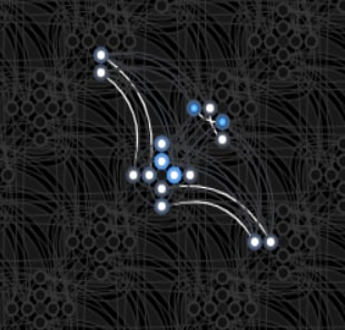
\includegraphics[width=5cm]{LaTeXTemplate/Images/AdvantageN10.png}
\caption{N=10\\max chain length = 2\\max chain strength=100.40\\physical qubits = 16}
\end{minipage}
\ \hspace{2mm} \hspace{2mm} \
\begin{minipage}[b]{4.5cm}
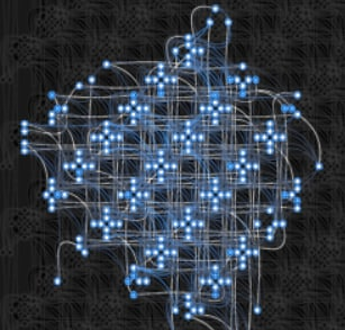
\includegraphics[width=5cm]{LaTeXTemplate/Images/AdvantageN40.png}
\caption{N=40\\max chain length = 7\\max chain strength=114.09\\physical qubits = 206}
\end{minipage}
\ \hspace{2mm} \hspace{2mm} \
\begin{minipage}[b]{4.5cm}
\centering
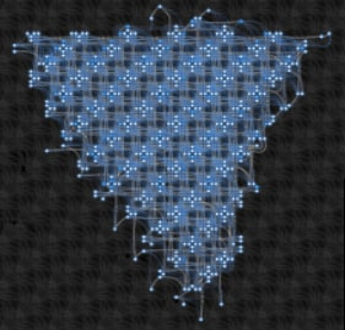
\includegraphics[width=5cm]{LaTeXTemplate/Images/AdvantageN70.png}
\caption{N=70\\max chain length = 11\\max chain strength=1839.2\\physical qubits = 553}
\end{minipage}
\end{figure}
\begin{figure}[htp]
\begin{minipage}[b]{4.5cm}
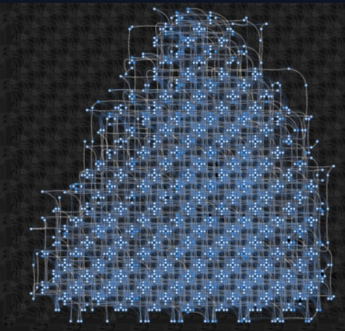
\includegraphics[width=5cm]{LaTeXTemplate/Images/AdvantageN100.png}
\caption{N=100\\max chain length = 19\\max chain strength=2722.5\\physical qubits = 1324}
\end{minipage}
\ \hspace{2mm} \hspace{2mm} \
\begin{minipage}[b]{4.5cm}
\centering
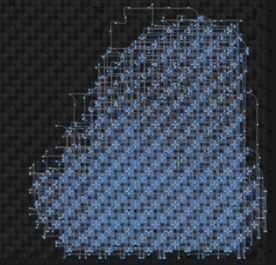
\includegraphics[width=5cm]{LaTeXTemplate/Images/AdvantageN130.png}
\caption{N=130\\max chain length = 28\\max chain strength=3011.2\\physical qubits = 2356}
\end{minipage}
\ \hspace{2mm} \hspace{2mm} \
\begin{minipage}[b]{4.5cm}
\centering
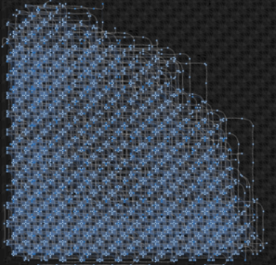
\includegraphics[width=5cm]{LaTeXTemplate/Images/AdvantageN150.png}
\caption{N=150\\max chain length=34\\max chain strength=2350.4\\physical qubits=3309}
\end{minipage}
\end{figure}

\newpage
In order to evaluate the time complexity,with the same aforementioned settings, we chose to repeat the experiment ten times. Then we made the average of the results achieved in order to collect a more reliable result. Thanks to leap we could print on a file several data about timing and energy and using python script we obtained the following results:\\
\\
\textbf{2000Q}
\begin{figure}[htp]
\begin{minipage}[b]{7.5cm}
\centering
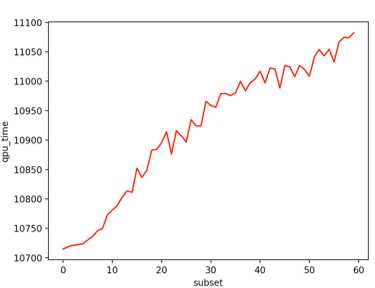
\includegraphics[width=9cm]{LaTeXTemplate/Images/2000QTimeComplexity.png}
\caption{2000Q Time complexity: mean}
\end{minipage}
\ \hspace{2mm} \hspace{2mm} \
\begin{minipage}[b]{9cm}
\centering
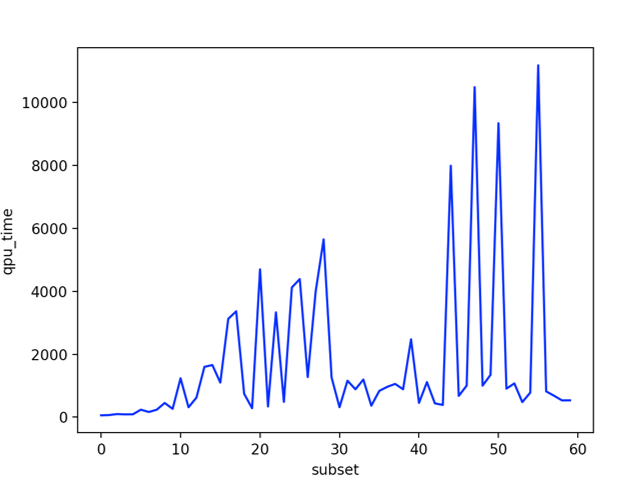
\includegraphics[width=9cm]{LaTeXTemplate/Images/2000QTimeVariance.png}
\caption{2000Q Time complexity: variance}
\end{minipage}
\end{figure}\\
As it can be noticed in figures 29 and 30, the mean and variance of the QPU time has been computed for each value of $N$. The resulting mean increases as a function of the number of subsets defined in the problem. The variance increases as well, even though more irregularly.

\newpage
\begin{figure}[htp]
\begin{minipage}[b]{7.5cm}
\centering
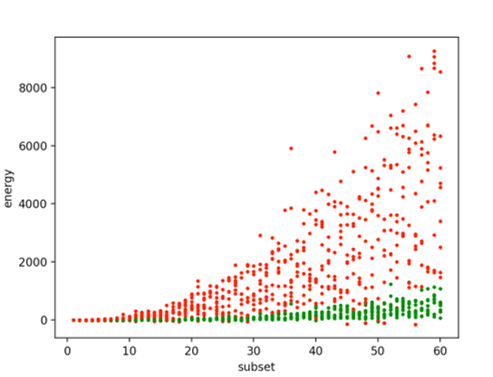
\includegraphics[width=9cm]{LaTeXTemplate/Images/2000QMaxMinEnValue.png}
\caption{2000Q Max and min energy:values}
\end{minipage}
\ \hspace{2mm} \hspace{2mm} \
\begin{minipage}[b]{9cm}
\centering
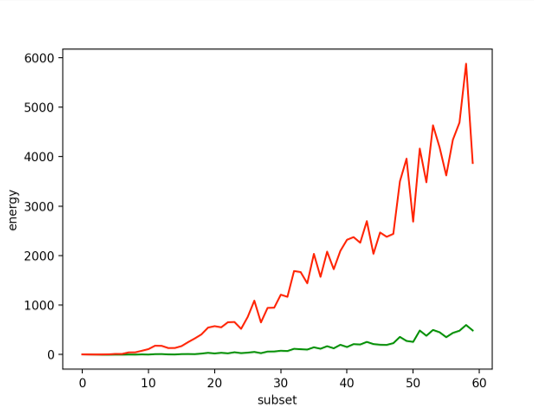
\includegraphics[width=9cm]{LaTeXTemplate/Images/2000QMaxMinEnMean.png}
\caption{Max and min energy: mead}
\end{minipage}
\end{figure}
For what concerns the maximum and minimum value of energy, for each value of $N$, it can be seen that the mean value for the minimum energy remains approximately constant, while the maximum value increases as a function of $N$. \\
\\
\textbf{Advantage}

\begin{figure}[htp]
\begin{minipage}[b]{7.5cm}
\centering
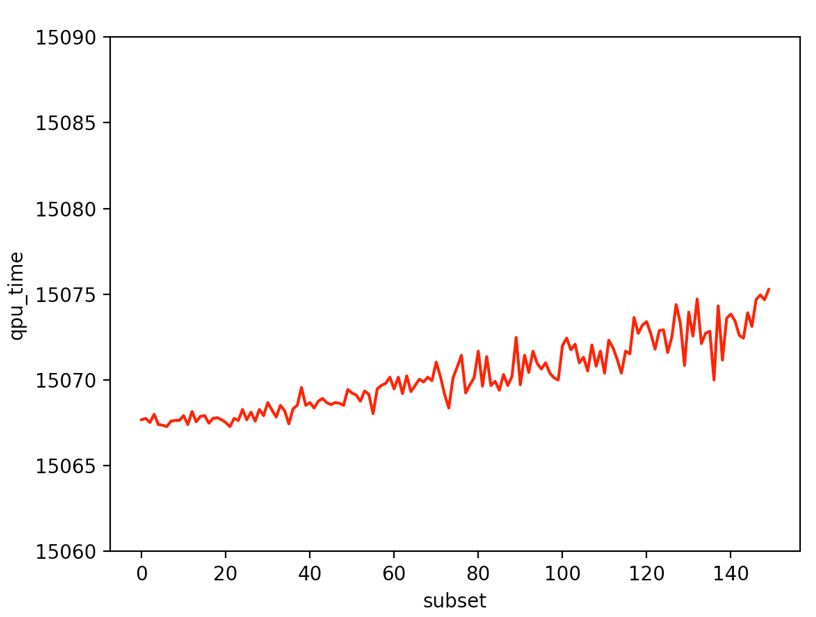
\includegraphics[width=8cm]{LaTeXTemplate/Images/AdvantageTimeComplexity.png}
\caption{Advantage Time complexity: mean}
\end{minipage}
\ \hspace{2mm} \hspace{2mm} \
\begin{minipage}[b]{9cm}
\centering
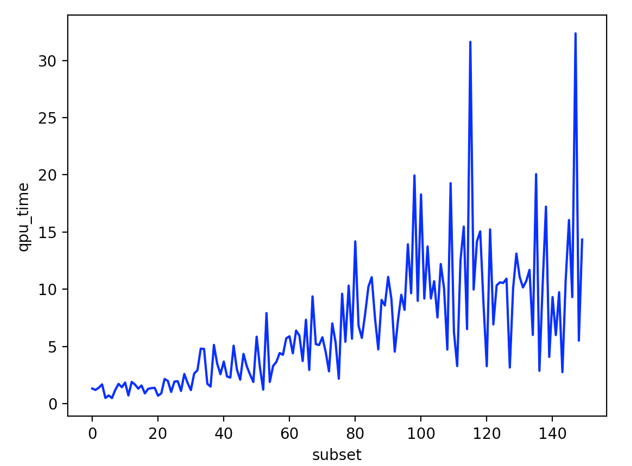
\includegraphics[width=8cm]{LaTeXTemplate/Images/AdvantageTimeVariance.png}
\caption{Advantage Time complexity: variance}
\end{minipage}
\end{figure}

As it can be noticed in figures 33 and 34, the mean of the ten execution has been calculated for each $N$. The resulting mean increases as a function of the number of subsets while the variance increases as well, even though more irregularly. In the following pictures, instead, the max and min energy is shown.
\newpage
\begin{figure}[htp]
\begin{minipage}[b]{9cm}
\centering
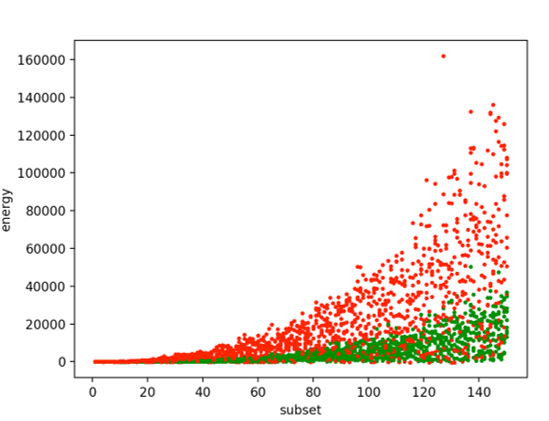
\includegraphics[width=9cm]{LaTeXTemplate/Images/MaxMinAdvValues.png}
\caption{Advantage Max and min energy:values}
\end{minipage}
\ \hspace{2mm} \hspace{2mm} \
\begin{minipage}[b]{9cm}
\centering
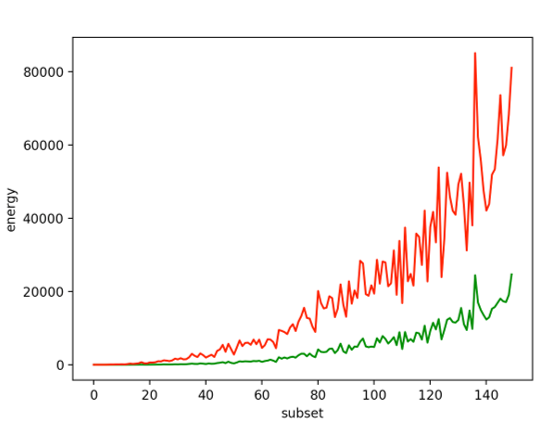
\includegraphics[width=9cm]{LaTeXTemplate/Images/MaxMinAdvMean.png}
\caption{Max and min energy: mean}
\end{minipage}
\end{figure}

For what concerns the maximum and minimum values of the energy, as it can be noticed in figures 35 and 36, the minimum energy increases as a function of $N$, as the maximum energy does, but the former rises significantly slower than the latter.

\section{Comparison}
\section{Conclusions}

\bibliographystyle{plain}
\bibliography{refs.bib}
\end{document}
